\documentclass{beamer}
\RequirePackage{luatex85}
\include{../style/cours-style.sty}

% Title
\title{Introduction au Développement Web - Bachelor CSI}
\author{Christophe Brun}
\institute{Campus Saint-Michel IT}
\date{25 juin 2024}
\beamertemplatenavigationsymbolsempty

\titlegraphic{
    \bigbreak
    
\includegraphics[width=2cm]{image/logo-papit}
    
\includegraphics[width=2cm]{image/logo-campus-saint-michel-it}
}
\begin{document}

    \begin{frame}
        \titlepage
        \bigbreak
        \centering
        \url{https://github.com/St-Michel-IT/Intro-dev-web}
    \end{frame}

    \begin{frame}{Table des matières}
        \tableofcontents
    \end{frame}


    \section{Programme du module}\label{sec:programme-du-module}
    \begin{frame}{Introduction au Développement Web}{Compétences}
        Programme officiel du module~:
        \begin{itemize}
            \item Réaliser une interface HTML/CSS
            \item Lire/Écrire/Modifier des données dans une base de données avec PHP
            \item Gérer un formulaire
        \end{itemize}
        \bigbreak
        Des remarques~?
    \end{frame}


    \section{Évaluation}\label{sec:evaluation}
    \begin{frame}{Évaluation}
        \begin{itemize}
            \item 60 \% sur les projets développés au cours du module.
            \begin{itemize}
                \item Basée en partie sur les commits des développements pour comprendre facilement l'évolution du code.
                \item Les exercices doivent être terminés dans les temps et les livrables dans Teams.
            \end{itemize}
            \item 40 \% sur une évaluation écrite finale.
        \end{itemize}
    \end{frame}

    \begin{frame}{Intervenant sur le module Introduction au Développement Web}{Christophe Brun, conseil en développement informatique}

        \begin{columns}
            \column{0.7\textwidth}
            \begin{itemize}
                \item 2\textsuperscript{nde} année d'intervenant à Saint-Michel \emoji{star-struck}.

                \item 7 ans de conseil en développement au sein d'SSII~.

                \item 7 ans de conseil en développement à mon compte \href{https://papit.fr}{PapIT}.

                \item Passionné~!
                \bigbreak
                \begin{columns}
                    \column{0.5\textwidth}
                    \centering
                    
\includegraphics[width=3cm]{image/logo-uppa}
                    \column{0.5\textwidth}
                    \centering
                    
\includegraphics[width=3cm]{image/logo-universite-bordeaux}
                \end{columns}
            \end{itemize}
            \column{0.3\textwidth}
            \centering
            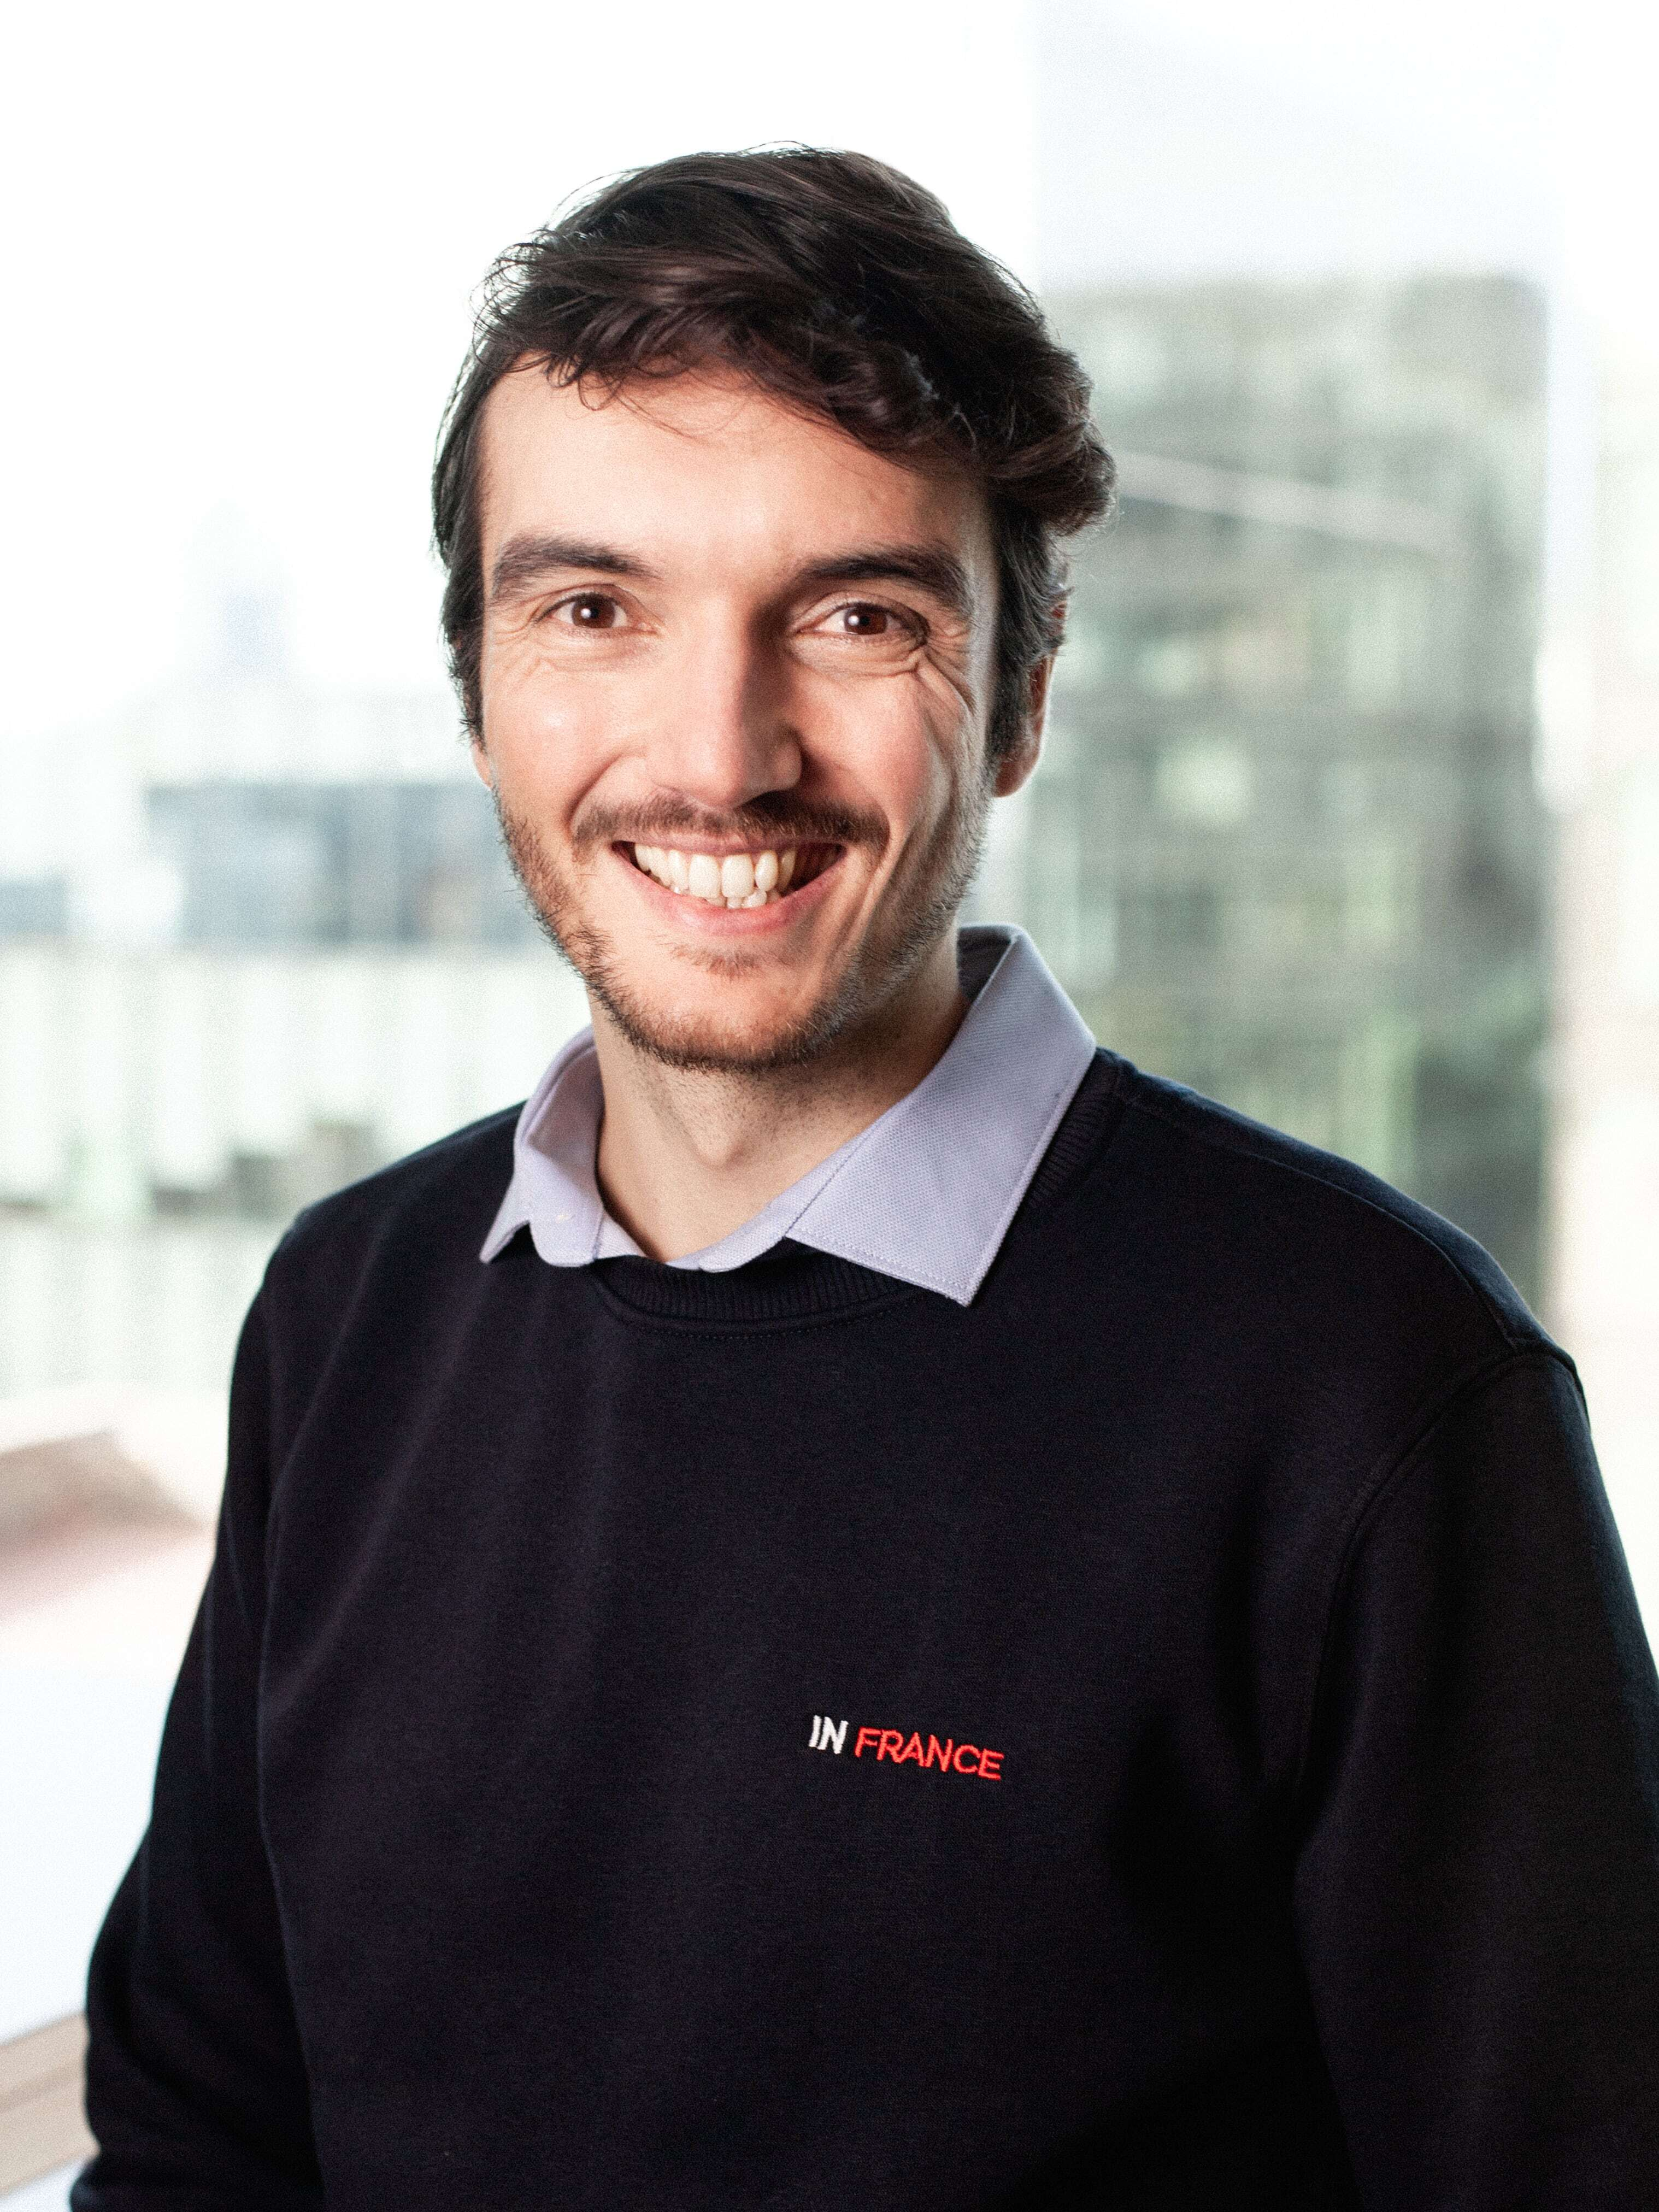
\includegraphics[width=5cm]{image/trombine-christophe}
        \end{columns}
    \end{frame}


    \section{Les ressources du Web}\label{sec:ressources}

    \begin{frame}{Les ressources du Web}{Dvisions en briques}
        \begin{columns}
            \column{0.6\textwidth}
            1 des 4 règles pour la direction de l'esprit de Descartes~: \textquote{Diviser chacune des difficultés que j'examinerais, en autant de parcelles qu'il se pourrait et qu'il serait requis pour les mieux résoudre.}.
            \column{0.4\textwidth}
            \centering
            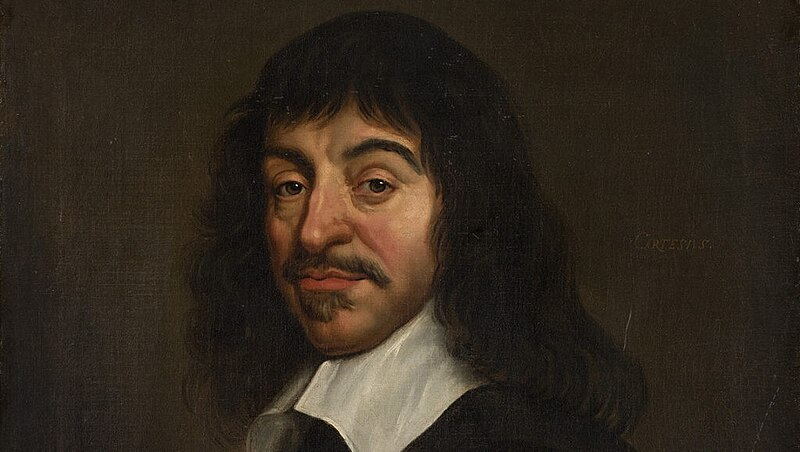
\includegraphics[width=6cm]{image/Descartes}
        \end{columns}
    \end{frame}

    \begin{frame}{Les ressources du Web}{Analyse des composants, exercice \execcounterdispinc}
        Listez toutes les ressources du Web que vous connaissez.
        \begin{itemize}
            \item ...
        \end{itemize}
        \bigbreak
        \begin{columns}
            \column{0.5\textwidth}
            Restituez-les dans un schéma au formalisme libre (Draw.io est conseillé\ldots).

            \textbf{Prenez le temps de bien nommer chaque concept.}
            \bigbreak
            À présenter au tableau~!
            \column{0.5\textwidth}
            \centering
            
\includegraphics[width=5cm]{image/computer-n-web-ressources}
        \end{columns}
    \end{frame}


    \section{Les protocoles du Web}\label{sec:protocoles}

    \begin{frame}{Les protocoles}{Introductions}
        \footnote{\label{sendbird-protocole}Protocoles de communication WebSocket vs. HTTP, \url{https://sendbird.com/fr/developer/tutorials/websocket-vs-http-communication-protocols}}
        Si on définit le Web comme les applications entre un navigateur et un serveur Web.
        \begin{dangercolorbox}
            Ce qui est très réducteur, car il ne prend pas en compte les applications mobiles, les API, les applications desktop, mail, etc.

            Mais c'est l'unique sujet de ce module\ldots
        \end{dangercolorbox}
        Quels sont les protocoles qui permettent à ces applications de communiquer~?
        \pause
        \bigbreak
        Il n'y en a que 2~!
        \begin{itemize}
            \item HTTP(S)
            \item Websocket
        \end{itemize}
    \end{frame}

    \begin{frame}{Les protocoles}{Introduction\label{sendbird-protocole}}
        HTTP, par contre, est un protocole de communication semi-duplex, qui existe depuis un certain temps et constitue la base du Web depuis ses débuts.

        HTTP date de 1989, inventé au CERN par Tim Berners-Lee\footnote{The birth of the Web, \url{https://home.cern/science/computing/birth-web}}.
        \bigbreak
        WebSocket, un protocole de communication full-duplex, est relativement plus récent et convient mieux aux applications en temps réel (ou presque\ldots) comme le live chat dans les applications mobiles, les notifications et ou les appels audio ou vidéo.

        Websocket a été standardisé en 2011\footnote{The WebSocket Protocol, \url{https://datatracker.ietf.org/doc/html/rfc6455}}.
        Il est géré par le Javascript du navigateur.
    \end{frame}

    \subsection{WebSocket}\label{subsec:websocket}

    \begin{frame}{Les protocoles}{Websocket, exercice \execcounterdispinc}
        \begin{itemize}
            \item Que veut dire full-duplex~?
            \item Y-a-t-il une contradiction avec une architecture client/serveur~?
            \item Citer un autre protocol full-duplex.
            \item Citer un protocol qui \textbf{n'est pas} full-duplex.
        \end{itemize}
        \bigbreak
        \centering
        
\includegraphics[width=5cm]{image/homework}
    \end{frame}

    \begin{frame}{Les protocoles}{Websocket\label{sendbird-protocole}}
        \centering
        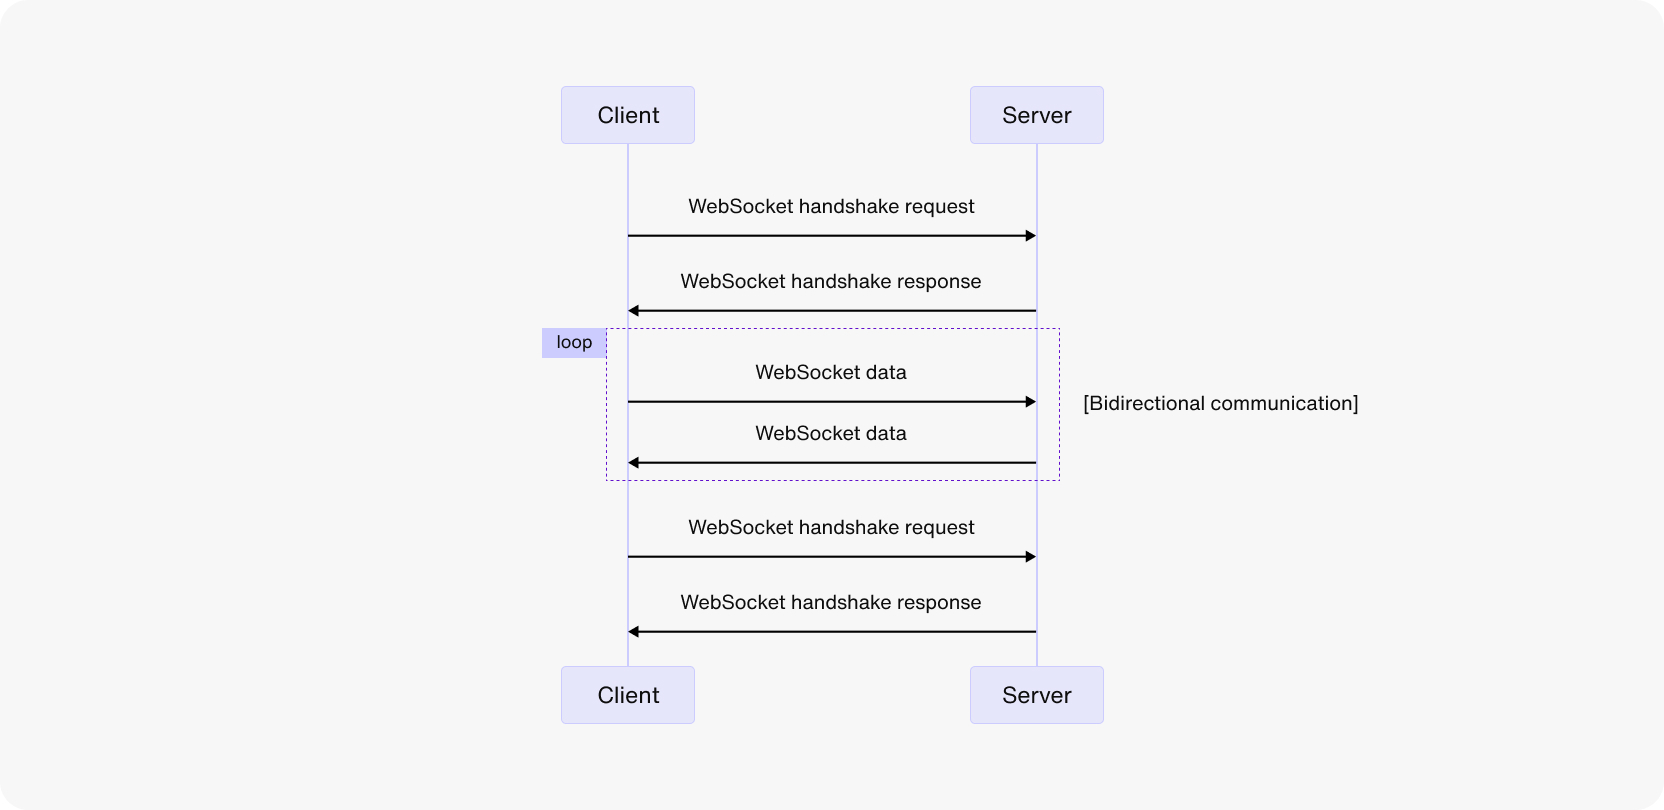
\includegraphics[width=12cm]{image/tutorial-websocket-protocol-chart}
    \end{frame}

    \begin{frame}{Les protocoles}{Websocket côté client (Navigateur)\footnote{\label{mozilla-websocket}WebSockets, \url{https://developer.mozilla.org/fr/docs/Web/API/WebSockets_API}}}
        \begin{columns}
            \column{0.5\textwidth}
            \centering
            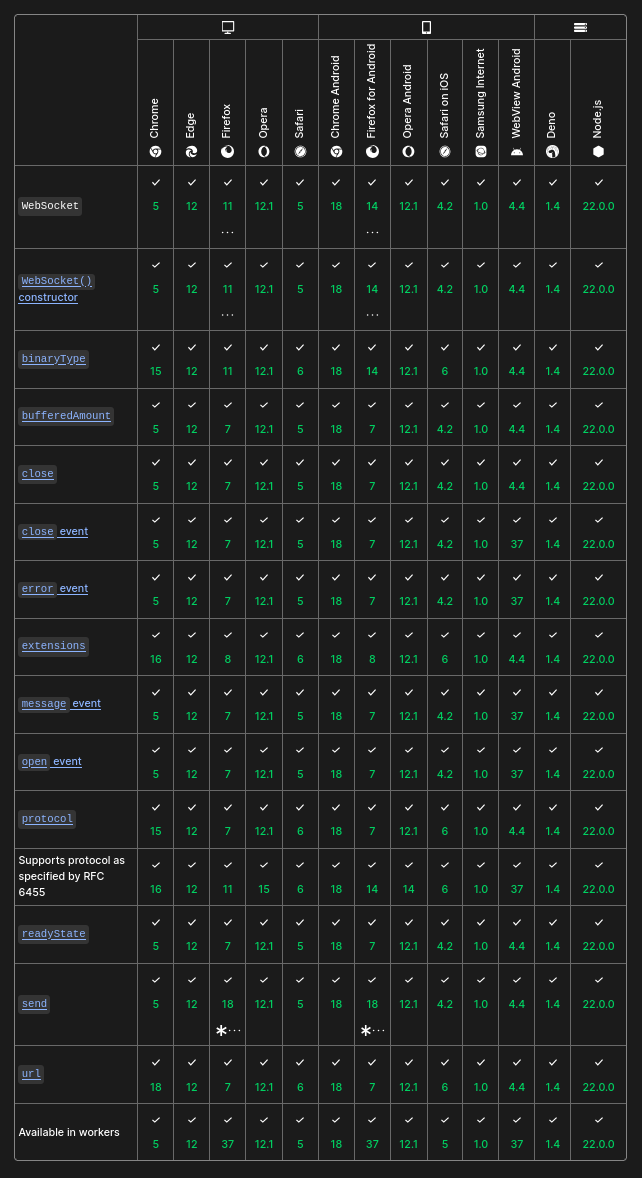
\includegraphics[width=3.3cm]{image/client-support} \\ Client \\
            \column{0.5\textwidth}
            \centering
            
\includegraphics[width=6.5cm]{image/kids-on-the-phone}
        \end{columns}
    \end{frame}

    \begin{frame}{Les protocoles}{Websocket côté serveur (liste non exhaustive !)\cref{mozilla-websocket}}
        \begin{scriptsize}
            \begin{itemize}

                \item \href{https://github.com/uWebSockets/uWebSockets}{µWebSockets}~: Déclinaison plus légère et plus performante de WebSocket et écrite en \href{https://isocpp.org/}{C++11} et en \href{https://nodejs.org/fr/}{Node.js}.

                \item \href{https://github.com/ClusterWS/ClusterWS}{ClusteWS~}: Framework léger, rapide et puissant qui permet de construire des applications en \href{https://nodejs.org/fr/}{Node.js}.

                \item \href{http://socket.io}{Socket.IO}~: API WebSocket puissante et multiplateforme en \href{https://nodejs.org}{Node.js}.

                \item \href{https://socketcluster.io/\#!/}{SocketCluster}~: Framework open source en temps réel en \href{https://nodejs.org}{Node.js}.

                \item \href{https://nodejs.org}{Node.js}.

                \item \href{https://www.totaljs.com/}{Total.js}~: FrameWork pour web application en \href{https://nodejs.org}{Node.js}.

                \item \href{https://www.npmjs.com/package/faye-websocket}{Faye}~: Combine WebSocket(bidirectionnelle) et EventSource(unidirectionnelle), côté serveur et côté client en \href{https://nodejs.org}{Node.js}.

                \item \href{https://signalr.net/}{SignalR}~: SignalR est une nouvelle bibliothèque pour les développeurs \href{https://dotnet.microsoft.com/apps/aspnet}{ASP.NET}.

                \item \href{https://caddyserver.com/docs/websocket}{Caddy}~: Serveur web capable de créer des WebSockets serveur/proxy(stdin/stdout, echo, cat, \ldots).

                \item \href{https://github.com/websockets/ws}{ws}~: La plus populaire des WebSockets pour client \& serveur en \href{https://nodejs.org}{Node.js}.

                \item \href{https://github.com/bigstepinc/jsonrpc-bidirectional}{jsonrpc-bidirectional}~: Implémentation de JSON-RPC 2.0 sur WebSocket.

                \item \href{https://github.com/ninenines/cowboy}{cowboy}~: Cowboy est un petit serveur HTTP rapide et moderne pour Erlang/OTP basé sur WebSocket.

                \item \href{https://zeromq.org}{ZeroMQ}~: ZeroMQ est une bibliothèque de fonctions pour transporter des messages avec divers protocoles IPC, TCP, UDP, TIPC, diffusion de groupe et WebSocket.

            \end{itemize}
        \end{scriptsize}
    \end{frame}

    \begin{frame}{Les protocoles}{Websocket, exercice \execcounterdispinc}
        Dans un groupe de deux ou trois~:
        \begin{itemize}
            \item Développer une page HTML avec un Javascript se connectant à un serveur WebSocket avec la techno/librairie de votre choix.
            \item Développer un serveur WebSocket avec la techno/librairie de votre choix.
            \item Les livrables, codes source \textbf{commentés} et captures d'écran, sont à déposer dans Teams.
        \end{itemize}
        \begin{dangercolorbox}
            À la vue de l'omniprésence de ce protocole sur de nombreuses technos et de la bonne compatibilité des méthodes.
            Est-il nécessaire d'utiliser des librairies (dépendances logicielles)~?
        \end{dangercolorbox}
    \end{frame}

    \subsection{HTTP}\label{subsec:http}

    \begin{frame}{Les protocoles}{HTTP\label{sendbird-protocole}}
        \centering
        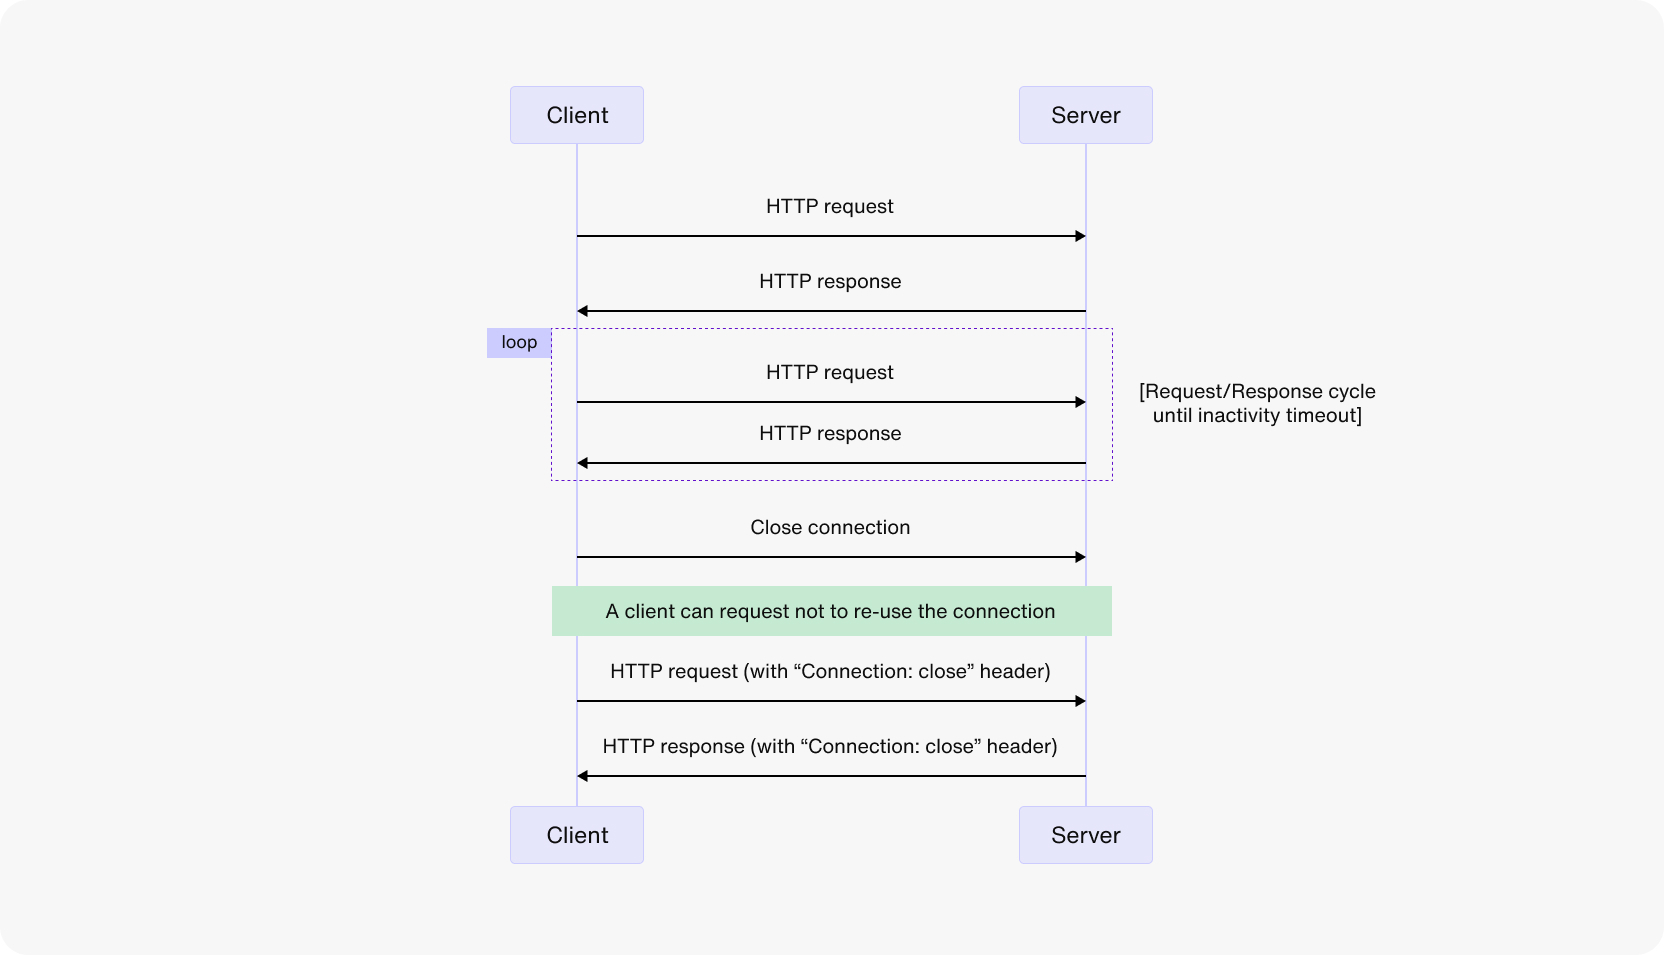
\includegraphics[width=12cm]{image/Tutorial-HTTP-connection-chart}
    \end{frame}

    \subsection{WebSocket VS HTTP}\label{subsec:ws-vs-http}

    \begin{frame}{Les protocoles}{HTTP\label{sendbird-protocole}}
        \centering
        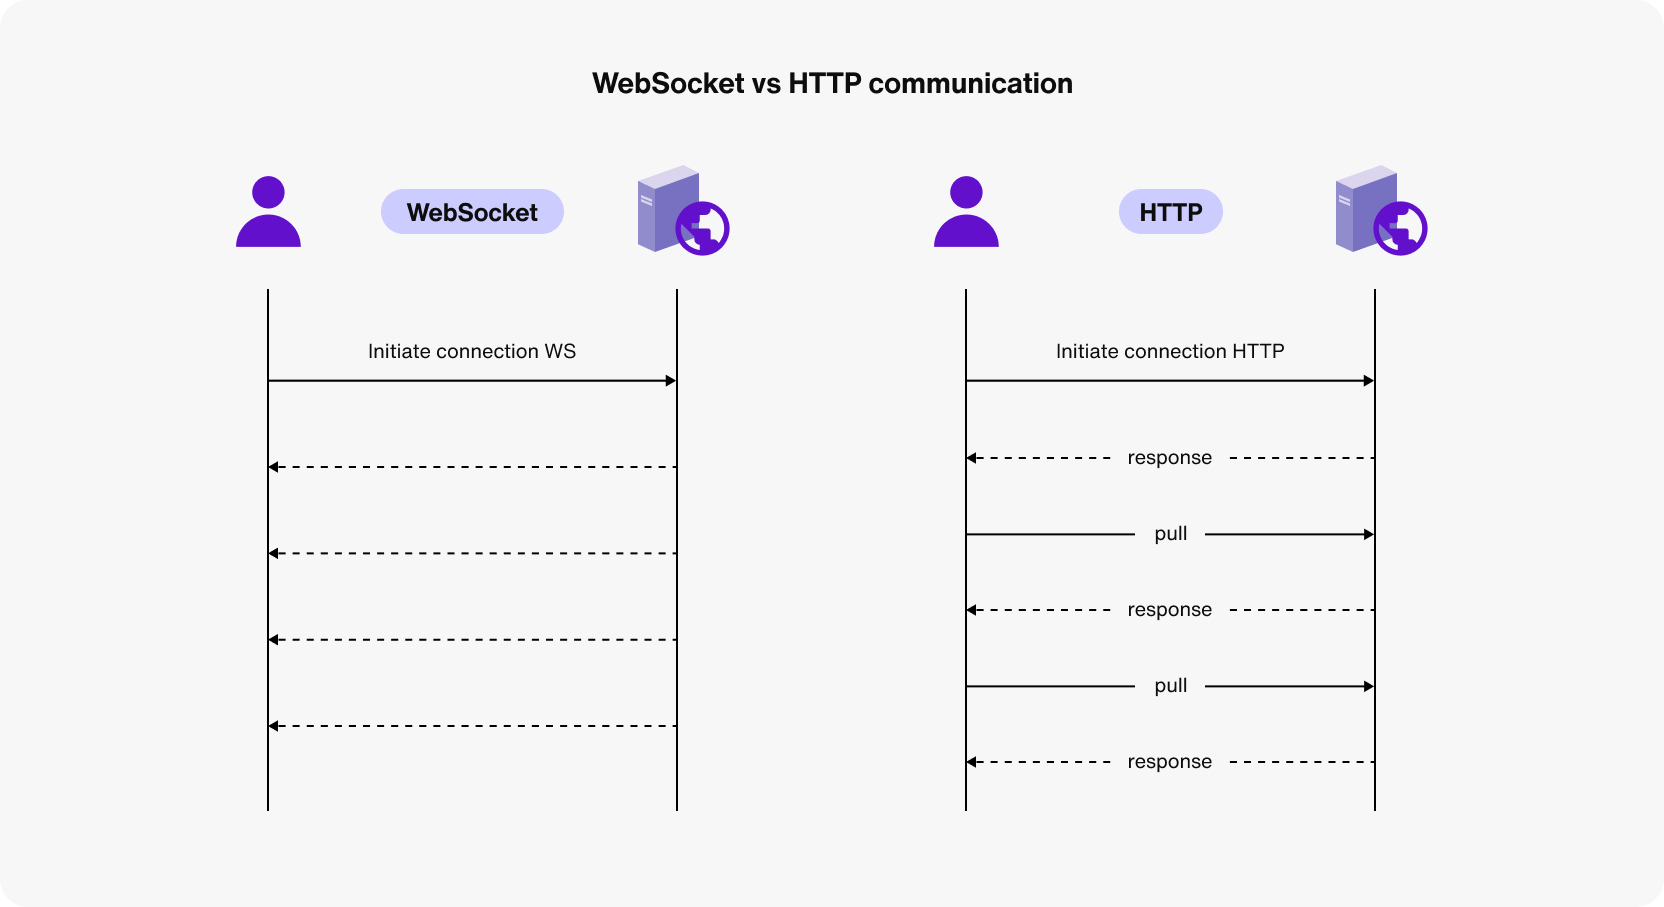
\includegraphics[width=12cm]{image/Tutorial-WebSocket-vs.-HTTP-communication-diagram}
    \end{frame}

    \begin{frame}{HTTP}{Introduction aux méthodes HTTP\footnote{\label{mozilla-http-methods}Méthodes de requête HTTP, \url{https://developer.mozilla.org/fr/docs/Web/HTTP/Methods}}}
        \begin{itemize}
            \item HTTP définit des méthodes de requête pour interagir avec les ressources.
            \item Ces méthodes sont souvent appelées \textit{verbes HTTP}.
            \item Les méthodes partagent parfois des fonctionnalités comme la \textit{sécurité}, l'\textit{idempotence}, ou la possibilité d'être \textit{mise en cache}.
        \end{itemize}
    \end{frame}

    \begin{frame}{HTTP}{Méthodes courantes\cref{mozilla-http-methods}}
        \begin{itemize}
            \item \lstinline{GET} : Récupère une ressource, sans modifier l'état du serveur (idempotence).
            Autorisée dans les \lstinline{<form>} HTML.
            \item \lstinline{HEAD} : Similaire à \lstinline{GET}~, sans le corps de la réponse.
            \item \lstinline{POST} : Envoie des données, créant ou modifiant une ressource.
            Autorisée dans les \lstinline{<form>} HTML.
            \item \lstinline{PUT} : Remplace la ressource avec les données envoyées.
            \item \lstinline{DELETE} : Supprime une ressource.
        \end{itemize}
        \begin{dangercolorbox}
            \lstinline{POST} et \lstinline{PUT} sont compatibles avec les formulaires, mais à quoi donc servent alors les autres~?
        \end{dangercolorbox}
    \end{frame}

    \begin{frame}{HTTP}{Autres méthodes\cref{mozilla-http-methods}}
        \begin{itemize}
            \item \lstinline{CONNECT} : Établit un tunnel vers le serveur cible.
            \item \lstinline{OPTIONS} : Renvoie les options de communication avec la ressource.
            \item \lstinline{TRACE} : Effectue un test aller-retour sur le chemin suivi.
            \item \lstinline{PATCH} : Applique des modifications partielles à une ressource.
        \end{itemize}
    \end{frame}

    \begin{frame}{HTTP}{Les URLs\footnote{Top REST API URL naming convention standards, \url{https://www.theserverside.com/video/Top-REST-API-URL-naming-convention-standards}}}
        \begin{tiny}
            Guidelines API REST~:
            \begin{itemize}
                \item Utilisez uniquement des lettres minuscules dans les URLs des API RESTful.
                \item Pour les espaces, utilisez kebab-case, et non snake\_case ou des espaces.
                \item Construisez les URIs avec des noms, pas des verbes.
                \item Utilisez les méthodes HTTP appropriées pour effectuer une opération.
                \item Les appels d'API REST qui retournent une collection doivent être au pluriel.
                \item Une URL qui retourne un résultat unique doit être au singulier.
                \item N'incluez pas d'extensions de fichier.
                \item Utilisez les en-têtes pour garder les URIs propres.
                \item N'identifiez pas les opérations de création, lecture, mise à jour et suppression (CRUD) dans l'URL~.
                \item Structurez les URIs librement selon la hiérarchie de votre modèle de données.
                \item Utilisez des paramètres de requête pour le filtrage et la recherche.
                \item Ne dévoilez pas le fonctionnement interne de votre architecture.
                \item Faites des URLs courtes, intuitives et lisibles.
                \item Protégez-vous contre les injections SQL~.
                \item Incluez la version de l'API REST à la base de l'URI~.
            \end{itemize}
        \end{tiny}
    \end{frame}

    \begin{frame}{HTTP}{Introduction à Content-Type\footnote{\label{mozilla-content-type}Content-Type, \url{https://developer.mozilla.org/fr/docs/Web/HTTP/Headers/Content-Type}}}
        \begin{itemize}
            \item \textbf{Content-Type} : Indique le type MIME de la ressource.
            \item Utilisé dans les réponses pour informer le client du type de contenu renvoyé.
            \item Utilisé dans les requêtes POST/PUT pour indiquer au serveur le type de données envoyées.
        \end{itemize}
        \bigbreak
        Pourquoi pas dans les GET~?

        La donnée est toujours dans l'URL et non dans le corps de la requête comme pour le POST.
        C'est donc inutile.
    \end{frame}

    \begin{frame}{HTTP}{Directives de Content-Type\cref{mozilla-content-type}}
        \begin{itemize}
            \item \lstinline{media-type} : Type MIME des données.
            \item \lstinline{charset} : Encodage des caractères.
            \item \lstinline{boundary} : Limites pour les entités multipart.
        \end{itemize}
    \end{frame}

    \begin{frame}[fragile]{HTTP}{Exemple : Formulaires HTML\cref{mozilla-content-type}}
        \begin{lstlisting}[language=HTML]
<form action="/" method="post" enctype="multipart/form-data">
  <input type="text" name="description" value="du texte" />
  <input type="file" name="monFichier" />
  <button type="submit">Envoyer</button>
</form>
        \end{lstlisting}
        \begin{itemize}
            \item Requête POST envoyée avec Content-Type multipart/form-data.
        \end{itemize}
        \begin{lstlisting}[language=HTML]
<form action="/recherche" method="get">
    <input type="text" name="q" value="recherche" />
    <button type="submit">Rechercher</button>
</form>
        \end{lstlisting}
        \begin{itemize}
            \item Requête GET envoyée avec Content-Type application/x-www-form-urlencoded.
        \end{itemize}

    \end{frame}


    \begin{frame}{Tableau des codes de statut HTTP\footnote{Codes de réponse HTTP, \url{https://developer.mozilla.org/fr/docs/Web/HTTP/Status}}}
        \begin{tabular}{|p{1.5cm}|p{9.5cm}|}
            \hline
            \textbf{Code} & \textbf{Description}                                                      \\
            \hline
            100-199       & Réponses informatives (e.g. 100 Continue, 101 Switching Protocols)        \\
            \hline
            200-299       & Succès (e.g. 200 OK, 201 Created)                                         \\
            \hline
            300-399       & Redirections (e.g. 301 Moved Permanently, 302 Found)                      \\
            \hline
            400-499       & Erreurs client (e.g. 400 Bad Request, 404 Not Found)                      \\
            \hline
            500-599       & Erreurs serveur (e.g. 500 Internal Server Error, 503 Service Unavailable) \\
            \hline
        \end{tabular}
    \end{frame}


    \begin{frame}{HTTP}{L'approche frameworkless}
        La plupart des langages comme Python ou Java viennent avec des libraires pour traiter les URL, les méthodes HTTP, les requêtes, \textit{etc}.
        \bigbreak
        \begin{itemize}
            \item Pourquoi, comment, expliquer le succès des frameworks webs~?
            \item  Quel(s) désavantage(s) ont les librairies natives~?
            \item  Quel(s) désavantage(s) ont les frameworks~?
        \end{itemize}
        \bigbreak
        Exercice \execcounterdispinc~: Développer un serveur HTTP en Python sans librairie tierce à partir de ce tutoriel \url{https://python.doctor/page-python-serveur-web-creer-rapidement}~.

        Le compléter avec tous les éléments vus précédemment, content-type, méthodes HTTP, URL.
    \end{frame}

    \begin{frame}{HTTP}{Le serveur web de 25 lignes}
        \centering
        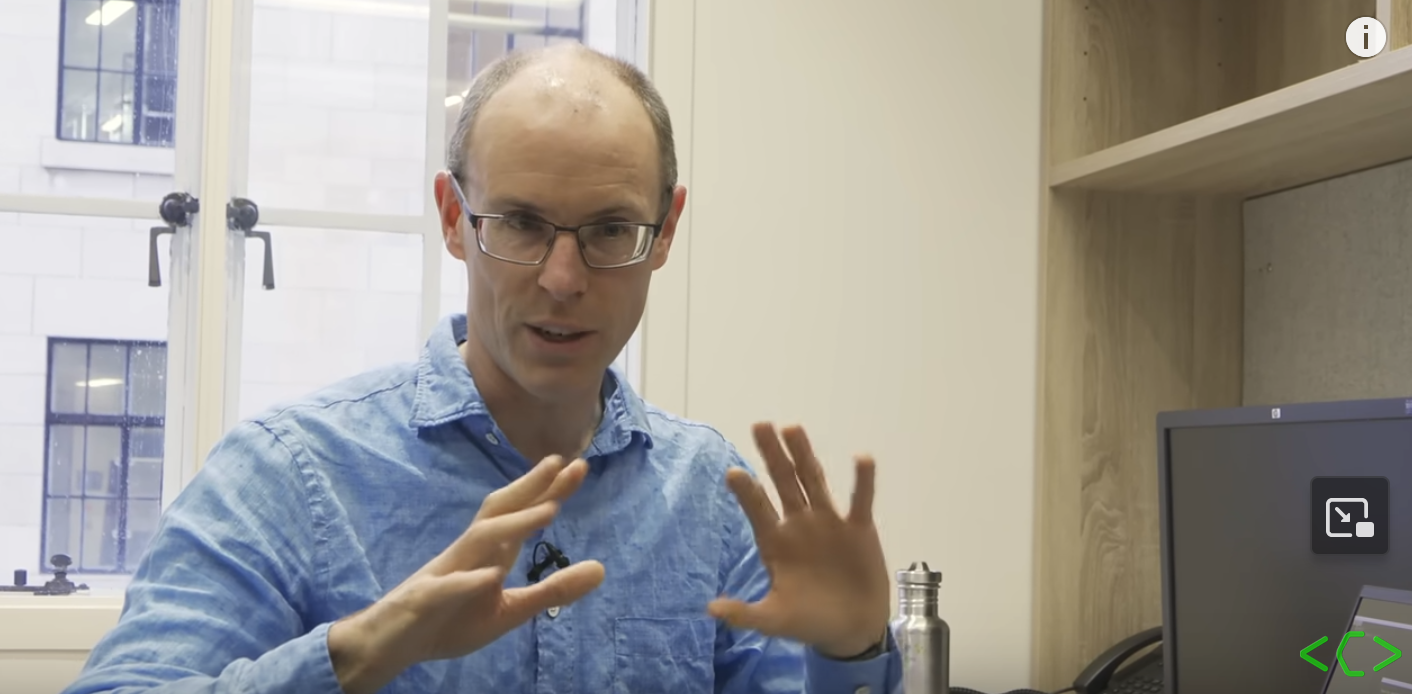
\includegraphics[width=12cm]{image/25-lines-server} \\ \url{https://www.youtube.com/watch?v=7GBlCinu9yg} \\
    \end{frame}


    \section{Licence CC}\label{sec:licence}

    \begin{frame}{Licence}{Licence Creative Commons}
        Support de cours sous licence Creative Commons BY-NC-ND~.
        \bigbreak
        Vous pouvez donc, partager, copier, distribuer le document.
        \bigbreak
        Attribution requise à PapIT SASU - Pas d’utilisation commerciale - Pas de modification
        \bigbreak
        \centering
        
\includegraphics[width=5cm]{image/by-nc-nd-logo}
    \end{frame}
\end{document}
